% -*- coding: UTF-8 -*-
% vim: autoindent expandtab tabstop=4 sw=4 sts=4 filetype=tex
% vim: spelllang=de spell
% chktex-file 27 - disable warning about missing include files

\section{Oberflächen}
\label{sec:surfaces}

Sofern im Text nicht anders vermerkt, basiert der folgende Abschnitt
auf~\cite[S. 1ff]{menon_introduction_1996}, sowie
auf~\cite[S. 79 bis 115]{glassner_introduction_1989}.

Für die Darstellung eines Bildes mittels Computergrafik, muss zunächst
definiert werden, was dargestellt werden soll. Dabei orientiert sich die
Computergrafik dabei an der realen Welt.  In dieser haben Oberflächen
von Objekten häufig keine starken Übergänge (Kanten) sondern sind eher
glatter Natur~\parencite[S.  471]{foley_computer_1996}.

Die Darstellung von Kurven und Oberflächen führt zu zwei Möglichkeiten:
Modellierung von bestehenden Objekten und Modellierung von Grund auf.

Zur Modellierung von Oberflächen werden hauptsächlich zwei Techniken verwendet:
Parametrische Modellierung und implizite Modellierung.

\subsection{Parametrische Darstellung von Oberflächen}
\label{subsec:surfaces:display:parametric}

Bei der parametrischen Darstellung wird eine Oberfläche üblicherweise als
eine Menge von Punkten definiert, so zum
Beispiel:

\begin{gather}\label{eq:surface_parametric}
    \bm{p}(s, t) = (x(s, t), y(s, t), z(s, t))
\end{gather}

So kann eine Kugel mittels sphärischen Koordinaten parametrisch
dargestellt werden wie folgt:

\begin{align}\label{eq:sphere_parametric}
    x(s, t) &= r \cdot \cos(s) \cdot \sin(t) \\
    y(s, t) &= r \cdot \sin(s) \cdot \sin(t) \\
    z(s, t) &= r \cdot \cos(t)
\end{align}

Dabei ist $r$ der Radius der Kugel, $s$ der Azimutwinkel $\in [0, 2\pi]$ und
$t$ der Polarwinkel $\in [0, \pi]$.

Die parametrische Darstellung bringt Vorteile wie Unabhängigkeit von
einem Koordinatensystem oder effiziente Berechnung von Punkten auf
einer Oberfläche.

\subsection{Implizite Darstellung von Oberflächen}
\label{subsec:surfaces:display:implicit}

Bei der impliziten Darstellung wird eine Oberfläche üblicherweise als Kontur
einer Funktion mit Wert 0 definiert~\parencite[S.
1]{menon_introduction_1996}, so zum Beispiel:

\begin{gather}\label{eq:surface_implicit}
    f(\bm{p}) = f(x, y, z) = 0
\end{gather}

Dabei ist $\bm{p}$ ein Punkt $(x, y, z)$ auf der Oberfläche, welche durch die Funktion
$f$ beschrieben wird.

Am Beispiel einer Kugel:

\begin{align}\label{eq:sphere_implicit}
    f(\bm{p}, r) = f(x, y, z, r) &= 0 \\
    f(\bm{p}, r) = \bm{p}^{2} - r^{2} &= 0 \\
    f(\bm{p}, r) = x^{2} + y^{2} + z^{2} - r^{2} &= 0
\end{align}

Dabei ist $\bm{p}$ ein Punkt $(x, y, z)$ auf der Oberfläche, welche durch
die Funktion $f$ beschrieben wird, und $r$ der Radius der Kugel
~\parencite[S. 91]{glassner_introduction_1989}.

Die implizite Darstellung erlaubt aus mathematischer Sicht eine grössere
Einflussnahme als die parametrische Darstellung und ist daher sehr
nützlich für Operationen wie Biegung, Vermischung, Schnitte
(Intersektion) oder Boolesche Operationen.

\subsection{Implizite Oberflächen}
\label{subsec:implicit_surfaces}

Wie in~\autoref{eq:surface_implicit} beschrieben, ist eine implizite
Oberfläche gemäss~\citeauthor{menon_introduction_1996} typischerweise als
Kontur einer Funktion mit Wert 0
definiert~\parencite[S. 1]{menon_introduction_1996}.
\citeauthor{hart_ray_1993} hingegen definiert eine implizite Oberfläche
als Funktion $ f(\bm{x}) = \mathbb{R}^{3} \to \mathbb{R} $. Jedem
Punkt einer Menge $ \bm{p} \in \mathbb{R}^{3} $ wird ein skalarer
Wert $ s \in \mathbb{R} $ zugewiesen. Dabei besteht die Oberfläche aus
der Menge von Punkten $ \bm{x} \equiv (x, y, z) \in \mathbb{R}^{3}
$~\parencite[S. 527]{hart_sphere_1994}.

Angenommen $ \bm{A} $ ist ein geschlossener Festkörper, welcher durch die
Funktion $f$ beschrieben wird, dann kann gemäss~\citeauthor{hart_ray_1993} Folgendes
angenommen werden:

\begin{align} \label{eq:surface_implicit_condition}
    x \in \overset{\circ}{\bm{A}} \Leftrightarrow f(\bm{x}) &< 0 \\
    x \in \partial \bm{A}         \Leftrightarrow f(\bm{x}) &= 0 \\
    x \in \mathbb{R}^{3} - \bm{A} \Leftrightarrow f(\bm{x}) &> 0
\end{align}

Dies bedeutet, dass sich ein Punkt $\bm{x}$:

\begin{itemize}
    \item{$\overset{\circ}{\bm{A}}$}\\
        Genau dann \textit{innerhalb} des Körpers $\bm{A}$ befindet,
        wenn die implizite Funktion $f(\bm{x})$ \textit{negativ} ist.
    \item $\partial{\bm{A}}$\\
        Genau dann \textit{auf der Oberfläche} des Körpers $\bm{A}$
        befindet, wenn die implizite Funktion $f(\bm{x})$ \textit{0}
        ist.
    \item $\mathbb{R}^{3} - \bm{A}$\\
        \textit{Nicht in oder auf} dem Körper $\bm{A}$ befindet, wenn
        die implizite Funktion $f(\bm{x})$ \textit{positiv} ist.
\end{itemize}

Obige Annahmen sind gültig, da es sich bei $ \bm{x} $ um eine Menge von Punkten mit topologischer
Struktur handelt~\parencite[S. 1]{hart_ray_1993}.

Gemäss~\citeauthor{menon_introduction_1996} finden hauptsächlich drei
Methoden zur Beschreibung impliziter Oberflächen Anwendung: Algebraische
Oberflächen, Blobby-Objekte sowie die funktionale
Repräsentation~\parencite[S.  1]{menon_introduction_1996}.\\
\citeauthor{hart_sphere_1994} gibt jedoch an, dass die gebräuchlichste
Form zur Darstellung von impliziten Oberflächen die algebraischen
Oberflächen sind~\parencite[S. 527]{hart_sphere_1994}. Diese werden
implizit durch polynomiale Funktionen definiert.

\subsubsection{Algebraische und geometrische implizite Oberflächen}
\label{ssubsec:implicit_surfaces_algebraic_geometric}

Ein Beispiel für eine algebraische Oberfläche ist die Beschreibung der
Einheitskugel anhand einer impliziten algebraischen Gleichung zweiten Grades:

\begin{gather} \label{eq:surface_immplicit_algebraic}
    x^{2} + y^{2} + z^{2} - r = 0\\
    x^{2} + y^{2} + z^{2} - 1 = 0
\end{gather}

Dabei hat Radius $r$ den Wert $1$, da es sich um die Einheitskugel
handelt.

\citeauthor{menon_introduction_1996} gibt an, dass algebraische Methoden
Oberflächen als implizite Polynome beschreiben.\\
So ist $F(x, y, y)$ beispielsweise ein Polynom in $x$, $y$ und
$z$~\parencite[S.  2]{menon_introduction_1996}.\\
Üblicherweise handelt es sich dabei um Polynome tiefen Grades (2, 3 oder
4)~\parencite[S.  2]{menon_introduction_1996}.\\
Die gebräuchlichsten Oberflächen sind quadratisch implizite Oberflächen
(vom Grad 2). Diese werden häufig als ``Quadrik'' (\textit{quadrics})
bezeichnet werden~\parencite[S.  2]{menon_introduction_1996}.

\citeauthor{hart_sphere_1994} gibt an, dass --- unter Nutzung einer Metrik ---
die Einheitskugel durch die implizite Gleichung geometrisch beschrieben
werden kann:

\begin{gather}\label{eq:surface_immplicit_geometric}
    \|\bm{x}\| - 1 = 0
\end{gather}

Unter Anwendung der allgemeinen Form einer impliziten Gleichung
(siehe~\autoref{eq:surface_implicit}) führt dies zu folgender Gleichung:

\begin{gather}\label{eq:surface_implicit_sphere}
    f(\bm{x}) = \|\bm{x}\| - 1
\end{gather}


Dabei ist $\|\bm{x}\|$ als euklidische Metrik definiert und entspricht
${(x^{2} + y^{2} + z^{2})}^{1 \over 2}$.

Die~\autoref{eq:surface_immplicit_algebraic} gibt die algebraische
Distanz zurück,~\autoref{eq:surface_immplicit_geometric} gibt die
geometrische Distanz zurück.

Gemäss~\citeauthor{hart_sphere_1994} wird die geometrische Darstellung
von quadrischen Oberflächen bevorzugt, da deren Parameter unabhängig von
Koordinaten und sie robuster und intuitiver sind.

Implizite Oberflächen werden bei Gleichungen der
Form~\ref{eq:surface_implicit_sphere} durch \textit{Distanzfunktionen}
repräsentiert. Diese messen oder binden
gemäss~\citeauthor{hart_sphere_1994} die geometrische Distanz zu deren
impliziten Oberflächen~\parencite[S. 529]{hart_sphere_1994}.

\subsubsection{Distanzfunktionen}
\label{ssubsec:distance_functions}

Wie anfangs erwähnt, definiert~\citeauthor{hart_sphere_1994} die
allgemeine Form zur Beschreibung bzw. Darstellung von impliziten
Oberflächen als Zuweisung von Punkten zu einem skalaren Wert: $ f :
\mathbb{R}^{n} \to \mathbb{R} $~\parencite[S. 527]{hart_sphere_1994}.

Unter Anwendung der unter~\autoref{eq:surface_implicit_condition}
definierten Bedingungen kann geschlossen werden, dass eine Menge von
Punkten $A$ existiert, welche Teil von $\mathbb{R}^{n}$, also $A \subset
\mathbb{R}^{n}$ ist. Dies heisst, dass alle Punkte in $A$ die folgende
Bedingung erfüllen:

\begin{gather}
    A = \{ x : f(x) \leq 0 \}
\end{gather}

\citeauthor{hart_sphere_1994} liefert folgende zwei Definition, welche der
Beschreibung von Distanzfunktionen dienen.

\theoremstyle{definition}
\begin{definition}{\label{theo:point_to_set_distance}
    \textit{Point-to-set distance}}\\
    Die Distanz eines Punktes zu einer Menge von Punkten definiert die Distanz
    eines Punktes $ \bm{x} \in \mathbb{R}^{3} $ zu einer Menge von Punkten $A
    \subset \mathbb{R}^{3}$ als Distanz von $\bm{x}$ zum nächsten Punkt in $A$:

    \begin{gather}
        d(\bm{x}, \bm{A}) = \min_{\substack{\bm{y} \in \bm{A}}}(\|\bm{x} - \bm{y}\|)
    \end{gather}
\end{definition}

\theoremstyle{definition}
\begin{definition}{\label{theo:signed_distnace_bound}
    \textit{Signed distance bound}}\\ 
    Eine Funktion $ f : \mathbb{R}^{3} \to \mathbb{R} $ ist eine
    Vorzeichen abhängige Obergrenze ihrer impliziten Oberfläche $ f^{-1}(0)$,
    wenn gilt:

    \begin{gather}\label{eq:signed_distnace_bound}
        |f(\bm{x})| \leq d(\bm{x}, f^{-1}(0))
    \end{gather}
\end{definition}

Wenn die~\autoref{eq:signed_distnace_bound} für eine Funktion $f$
gilt, dann ist $f$ eine \textit{Vorzeichen abhängige Distanzfunktion
    (signed distance function)}.

\subsubsection{Distanzfelder (distance fields)}
\label{ssubsec:distance_fields}

Sofern im Text nicht anders vermerkt, basiert der folgende Abschnitt
auf~\cite{jones_3d_2006}.

Bei einem Distanzfeld handelt es sich um eine Repräsentation respektive
um eine Datenstruktur, bei welcher von jedem Punkt aus die geringste
Distanz zu einem beliebigen Objekt der Domäne bekannt ist.

Zusätzlich zu der Distanz können aus einem Distanzfeld andere Parameter,
wie beispielsweise die Richtung einer Oberfläche, abgeleitet werden.

Handelt es sich bei einem Distanzfeld um ein mit Vorzeichen behaftetes
Distanzfeld, so kann bei jedem Punkt bestimmt werden, ob er sich
innerhalb, ausserhalb oder genau auf einem Objekt befindet. Dies verhält
sich analog zu~\autoref{subsec:implicit_surfaces}.

Distanzfelder bilden somit die Grundlage der Algorithmen zur Darstellung
von impliziten Oberflächen. Siehe dazu
auch~\autoref{sec:rendering_implicit_surfaces}. Die
unter~\autoref{ssubsec:distance_functions} genannte~\textit{Point-to-set
    distance}-Funktion  liefert bereits die nächste Distanz zu einer
Menge von Punkten und somit auch zu Objekten ausgehend von einem Punkt
der Domäne.

\begin{figure}[H]
    \centering
    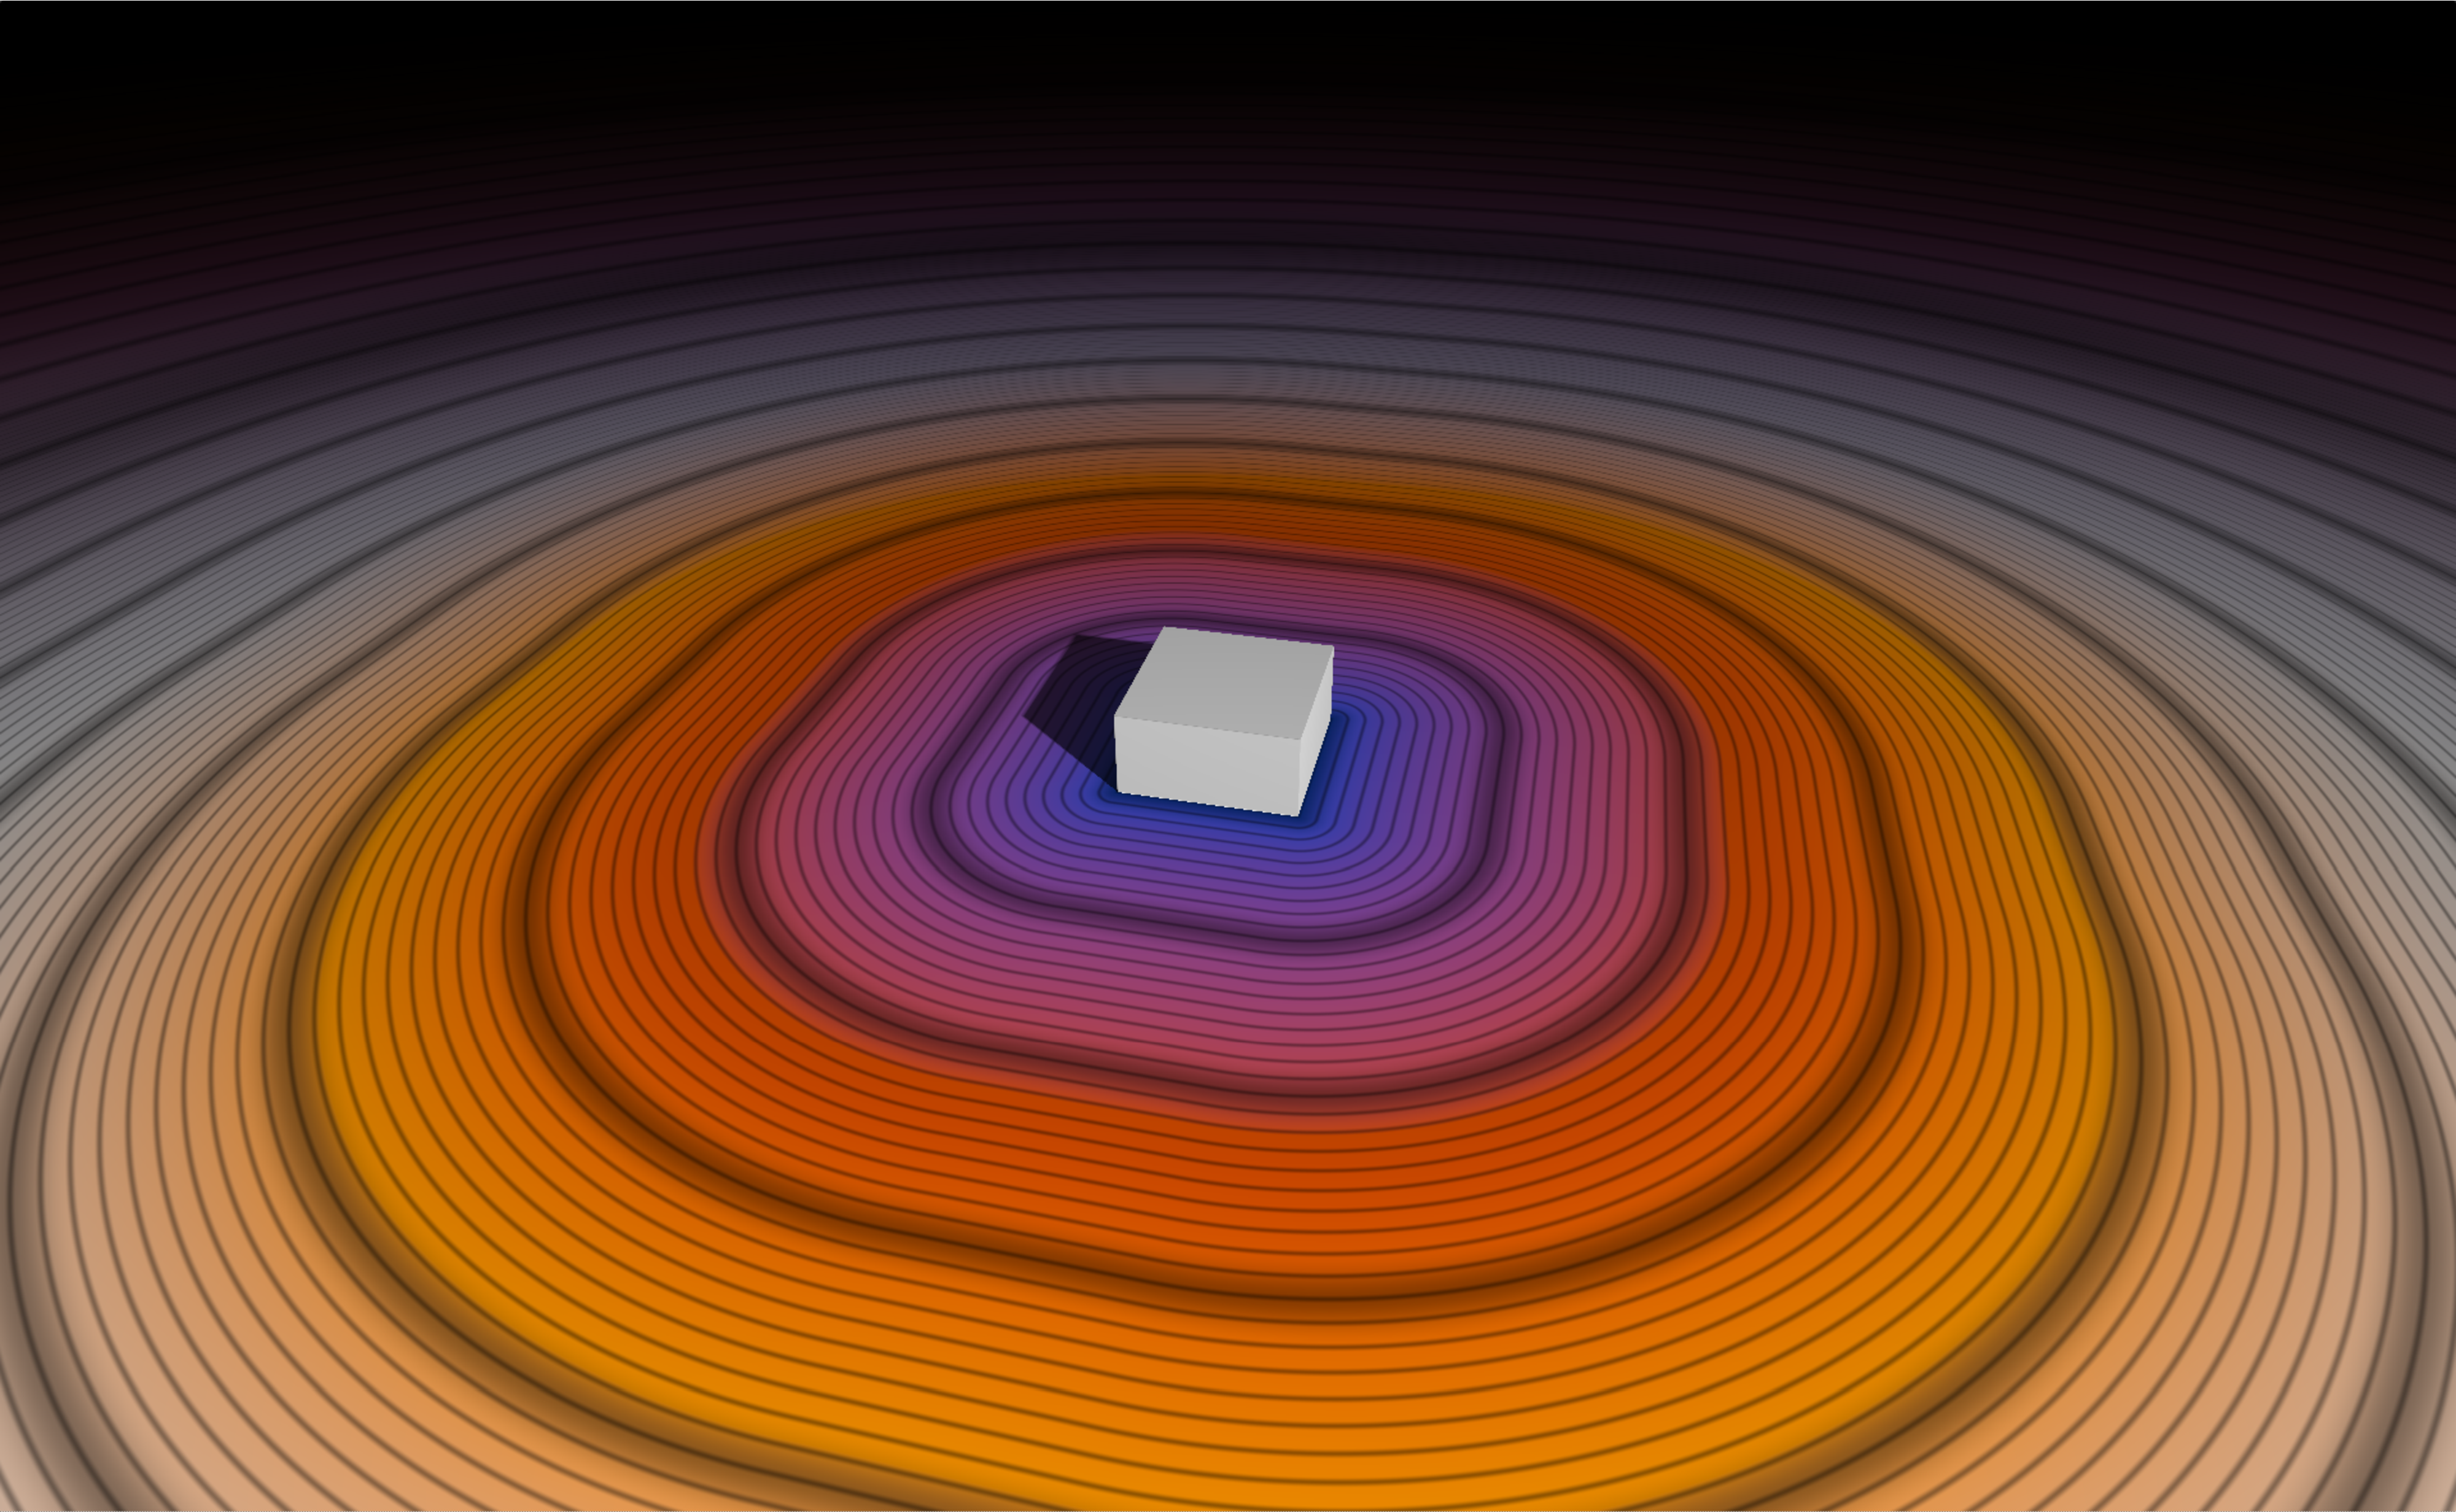
\includegraphics[width=0.5\textwidth]{img/distance_field.pdf}
    \caption{Darstellung des Distanzfeldes einer dreidimensionalen
        Szene anhand Farbwerten\protect\footnotemark}\label{
        fig:distance_field_illustration}
\end{figure}
\footnotetext{Eigene Darstellung}
